\documentclass{beamer}
\usepackage{graphicx}
\usepackage{xcolor}
\usepackage{tikz}
\usepackage{amsmath}

% 自定义颜色
\definecolor{purpleblue}{RGB}{80, 80, 180}
\definecolor{lightgray}{RGB}{230, 230, 230}
\definecolor{novelPurple}{RGB}{98, 54, 255} 
\definecolor{darkgray}{RGB}{50, 50, 50}

% 主题设置
\usetheme{Madrid}  
\usecolortheme{dolphin} 

% 设置字体
\setbeamerfont{title}{size=\Large,series=\bfseries}
\setbeamerfont{frametitle}{size=\LARGE,series=\bfseries}
\setbeamercolor{frametitle}{fg=white, bg=novelPurple}
\setbeamercolor{title}{fg=white, bg=purpleblue}

% 封面信息
\title[SAT Unit 1.5]{\textbf{SAT Unit 1.5 \\Linear Inequalities in One or Two Variables }}
\author{\textbf{Jack Zeng}}
\institute{\textcolor{white}{\textbf{Novel Prep}}}
\date{\today} 

\begin{document}

% --- Title Slide ---
\begin{frame}
    \titlepage
    \vfill
    \begin{flushright}
        \textcolor{purpleblue}{\Huge \textbf{Novel Prep}}
    \end{flushright}
\end{frame}

% --- Custom Background Slide ---
\begin{frame}
    \begin{tikzpicture}[remember picture, overlay]
        \shade[top color=softPurple, bottom color=softGray] 
            (current page.north west) rectangle (current page.south east);
        \fill[white, opacity=0.3] (current page.center) circle (4cm);
        \node[align=center] at (current page.center) {
            {\Huge\bfseries\textcolor{purpleblue}{Novel Prep}} \\[0.5cm]
            {\Large\itshape\textcolor{lightText}{Excellence in SAT Prep}}
        };
        \foreach \x in {1,2,3,4,5} {
            \fill[purpleblue, opacity=0.2] (rand*10-5, rand*7-3.5) circle (0.1+\x*0.05);
        }
        ;
    \end{tikzpicture}

\end{frame}


\begin{frame}{Overview}
    \tableofcontents
\end{frame}

\begin{frame}
\section{Solving Linear Inequalities (One Variable)}
    \begin{tikzpicture}[remember picture, overlay]
        \shade[top color=softPurple, bottom color=softGray] 
            (current page.north west) rectangle (current page.south east);
        \fill[white, opacity=0.3] (current page.center) circle (4cm);
        \node[align=center] at (current page.center) {
            {\LARGE\bfseries\textcolor{purpleblue}{Solving Linear Inequalities (One Variable)}} \\[0.5cm]
            {\Large\itshape\textcolor{lightText}{Excellence in SAT Prep}}
        };
        \foreach \x in {1,2,3,4,5} {
            \fill[purpleblue, opacity=0.2] (rand*10-5, rand*7-3.5) circle (0.1+\x*0.05);
        }
        ;
    \end{tikzpicture}

\end{frame}
% --- Slide: What is a Linear Inequality?
\begin{frame}{What is a Linear Inequality?}
    A linear inequality is similar to a linear equation, but instead of using $=$, it uses:
    \begin{itemize}
        \item $<$ (less than)
        \item $\le$ (less than or equal to)
        \item $>$ (greater than)
        \item $\ge$ (greater than or equal to)
    \end{itemize}

    \vspace{0.5cm}
    \textbf{Examples:}
    \[
    x + 2 < 5 \quad \text{or} \quad 2x - 3 \ge 7
    \]
    
\end{frame}

% --- Slide: Solving Linear Inequalities (One Variable)
\begin{frame}{Solving Linear Inequalities (One Variable)}
    \textbf{Steps:}
    \begin{enumerate}
        \item Isolate the variable on one side.
        \item Use inverse operations as with equations.
        \item Important: \textbf{Flip the inequality sign} when multiplying or dividing by a negative number!
    \end{enumerate}

    \vspace{0.5cm}
    \textbf{Example:}
    \[
    -3x + 2 \le 8 \Rightarrow -3x \le 6 \Rightarrow x \ge -2
    \]
\end{frame}

% --- Slide: Graphing on a Number Line
\begin{frame}{Graphing One-Variable Inequalities}
    \begin{itemize}
        \item Use an open circle for $<$ or $>$.
        \item Use a closed circle for $\le$ or $\ge$.
        \item Shade the direction of the inequality.
    \end{itemize}

    \vspace{0.5cm}
    \textbf{Example: } $x > 2$ is represented with an open circle at $2$ and shading to the right.
\end{frame}
\begin{frame}
\section{Linear Inequalities in Two Variables}
    \begin{tikzpicture}[remember picture, overlay]
        \shade[top color=softPurple, bottom color=softGray] 
            (current page.north west) rectangle (current page.south east);
        \fill[white, opacity=0.3] (current page.center) circle (4cm);
        \node[align=center] at (current page.center) {
            {\LARGE\bfseries\textcolor{purpleblue}{Linear Inequalities in Two Variables}} \\[0.5cm]
            {\Large\itshape\textcolor{lightText}{Excellence in SAT Prep}}
        };
        \foreach \x in {1,2,3,4,5} {
            \fill[purpleblue, opacity=0.2] (rand*10-5, rand*7-3.5) circle (0.1+\x*0.05);
        }
        ;
    \end{tikzpicture}
\end{frame}
% --- Slide: Linear Inequalities in Two Variables
\begin{frame}{Linear Inequalities in Two Variables}
\small
    A linear inequality in two variables looks like:
    \[
    Ax + By < C
    \quad \text{or} \quad
    Ax + By \ge C
    \]

    \textbf{Steps to graph:}
    \begin{enumerate}
        \item Rewrite as an equation to find the boundary line.
        \item Use a solid line for $\le$ or $\ge$, dashed for $<$ or $>$.
        \item Pick a test point (usually $(0,0)$) to determine shading side.
    \end{enumerate}

            \begin{center}
        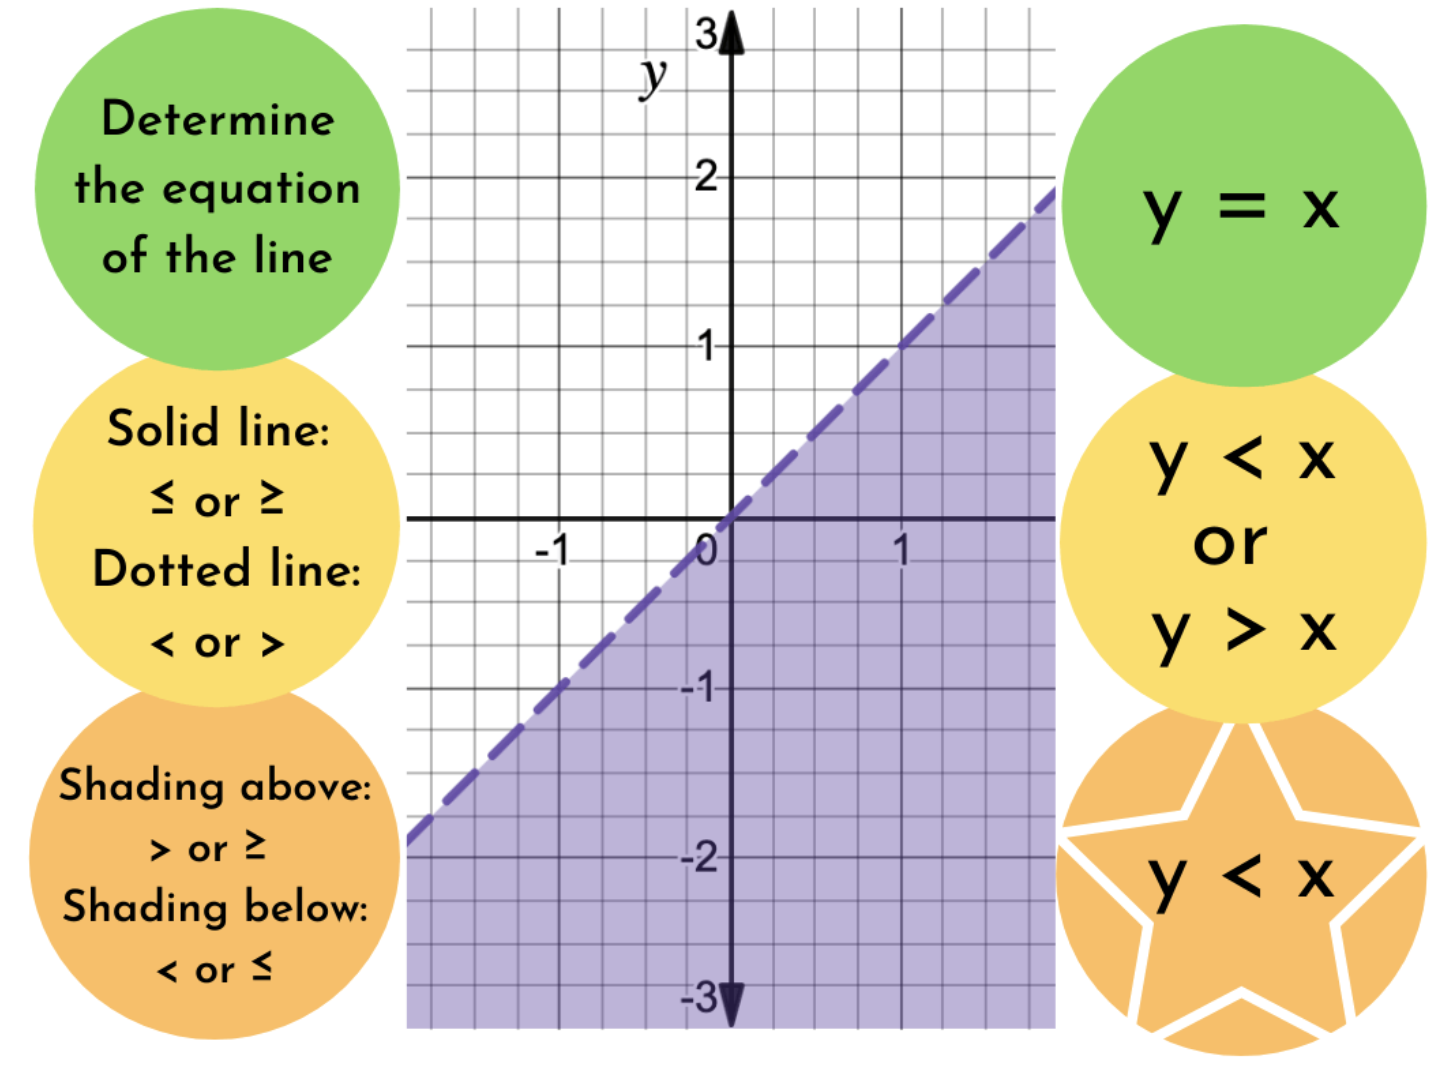
\includegraphics[width=0.5\linewidth]{E18.png}
    \end{center}
\end{frame}


% --- Slide: Graphing Example
\begin{frame}{Example: Graphing $y < 2x + 1$}

    \begin{itemize}
        \item Step 1: Graph the boundary line $y = 2x + 1$ (dashed line).
        \item Step 2: Test $(0,0)$: $0 < 2(0) + 1$ is true.
        \item Step 3: Shade the region below the line.
    \end{itemize}
    \vspace{0.3cm}
    This shaded region represents all the $(x, y)$ pairs that make the inequality true.

                \begin{center}
        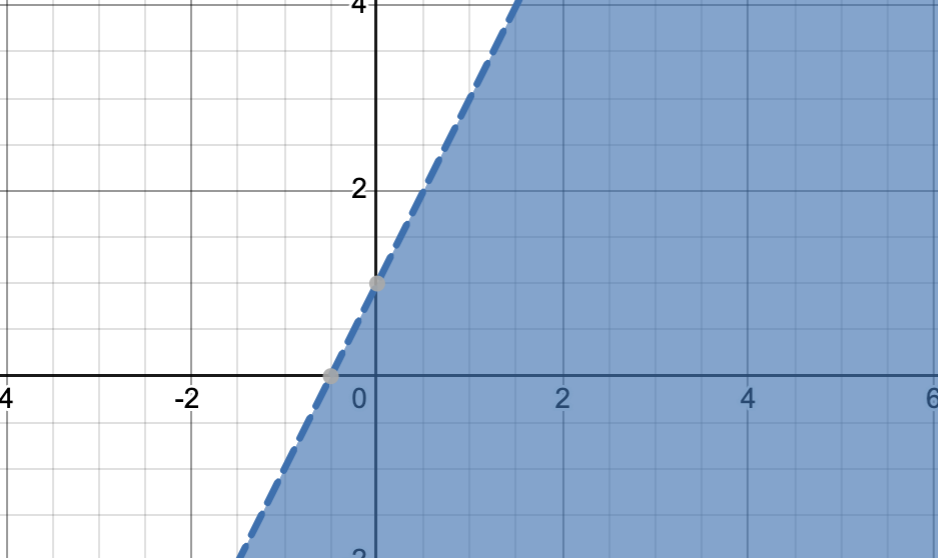
\includegraphics[width=0.6\linewidth]{E19.png}
    \end{center}


\end{frame}

\begin{frame}
\section{System of Linear Inequalities}
    \begin{tikzpicture}[remember picture, overlay]
        \shade[top color=softPurple, bottom color=softGray] 
            (current page.north west) rectangle (current page.south east);
        \fill[white, opacity=0.3] (current page.center) circle (4cm);
        \node[align=center] at (current page.center) {
            {\LARGE\bfseries\textcolor{purpleblue}{System of Linear Inequalities}} \\[0.5cm]
            {\Large\itshape\textcolor{lightText}{Excellence in SAT Prep}}
        };
        \foreach \x in {1,2,3,4,5} {
            \fill[purpleblue, opacity=0.2] (rand*10-5, rand*7-3.5) circle (0.1+\x*0.05);
        }
        ;
    \end{tikzpicture}
\end{frame}
% --- Slide: System of Linear Inequalities ---
\begin{frame}{System of Linear Inequalities}
\small
    A \textbf{system of linear inequalities} is a set of two or more linear inequalities with the same variables.


    \textbf{Solution:} The solution is the region where the shaded areas of all inequalities \textbf{overlap}.


    \textbf{Example:}
    \[
    \begin{cases}
    y \le 2x + 3 \\
    y > -x + 1
    \end{cases}
    \]

    \begin{itemize}
        \item Step 1: Graph each inequality on the same coordinate plane.
        \item Step 2: Use dashed or solid lines depending on the symbols ($<$ or $\le$).
        \item Step 3: Shade the region for each inequality.
        \item Step 4: The overlapping shaded region is the solution set.
    \end{itemize}
    \begin{center}
        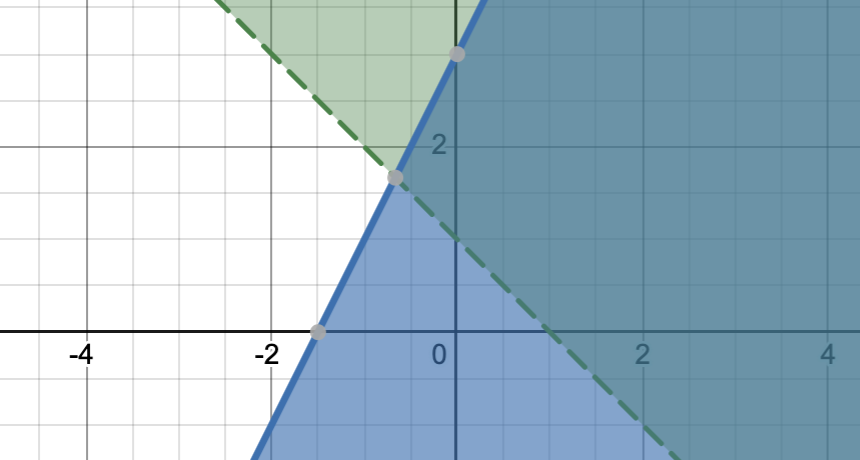
\includegraphics[width=0.35\linewidth]{E20.png}
    \end{center}
\end{frame}

\begin{frame}{Question: System of Inequalities}
    \small
    Given the system of inequalities:
    \[
    \begin{aligned}
        y &\leq x + 7 \\
        y &\geq -2x - 1
    \end{aligned}
    \]
    Which point $(x, y)$ is a solution to the system?

    \begin{itemize}
        \item[(A)] $(-14, 0)$
        \item[(B)] $(0, -14)$
        \item[(C)] $(0, 14)$
        \item[(D)] $(14, 0)$
    \end{itemize}
\end{frame}
\begin{frame}{Solution — Inequality System}
    \small
    Check each point to see which satisfies \emph{both} inequalities:
    \[
    y \leq x + 7 \quad \text{and} \quad y \geq -2x - 1
    \]

    \begin{itemize}
        \item \textbf{(A)} $x = -14,\ y = 0$:
        \[
        0 \leq -14 + 7 = -7 \quad \text{(False)} \quad \Rightarrow \text{Reject}
        \]

        \item \textbf{(B)} $x = 0,\ y = -14$:
        \[
        -14 \leq 0 + 7 = 7 \quad \text{(True)} \\
        -14 \geq -2(0) - 1 = -1 \quad \text{(False)} \quad \Rightarrow \text{Reject}
        \]

        \item \textbf{(C)} $x = 0,\ y = 14$:
        \[
        14 \leq 0 + 7 = 7 \quad \text{(False)} \quad \Rightarrow \text{Reject}
        \]

        \item \textbf{(D)} $x = 14,\ y = 0$:
        \[
        0 \leq 14 + 7 = 21 \quad \text{(True)} \\
        0 \geq -2(14) - 1 = -29 \quad \text{(True)} \quad \Rightarrow \text{Accept}
        \]
    \end{itemize}

    \textbf{Answer:} $\boxed{\text{D}}$
\end{frame}

\begin{frame}{Question: Inequality Table Matching}
    \small
    Given the inequality:
    \[
    y < 6x + 2
    \]
    For which of the following tables are \textbf{all} $(x, y)$ values solutions to the inequality?

\vspace{5mm}

    \begin{columns}
    \column{0.45\textwidth}
    \textbf{A.}
    \[
    \begin{array}{c|c}
    x & y \\
    \hline
    3 & 20 \\
    5 & 32 \\
    7 & 44 \\
    \end{array}
    \]

    \textbf{B.}
    \[
    \begin{array}{c|c}
    x & y \\
    \hline
    3 & 16 \\
    5 & 36 \\
    7 & 40 \\
    \end{array}
    \]

    \column{0.45\textwidth}
    \textbf{C.}
    \[
    \begin{array}{c|c}
    x & y \\
    \hline
    3 & 16 \\
    5 & 28 \\
    7 & 40 \\
    \end{array}
    \]

    \textbf{D.}
    \[
    \begin{array}{c|c}
    x & y \\
    \hline
    3 & 24 \\
    5 & 36 \\
    7 & 48 \\
    \end{array}
    \]
    \end{columns}
\end{frame}


\begin{frame}{Solution — Checking the Tables}
    \small
    The inequality is:
    \[
    y < 6x + 2
    \]

    \begin{itemize}
        \item For $x = 3$, $6x + 2 = 20$
        \item For $x = 5$, $6x + 2 = 32$
        \item For $x = 7$, $6x + 2 = 44$
    \end{itemize}

    \textbf{Compare each $y$ with the threshold values:}

    \begin{itemize}
        \item \textbf{A:} $y = 20, 32, 44$ → Not less than → ✗
        \item \textbf{B:} $y = 16 < 20$, $36 > 32$ ✗
        \item \textbf{C:} $y = 16 < 20$, $28 < 32$, $40 < 44$ → ✓
        \item \textbf{D:} $y = 24 > 20$ ✗
    \end{itemize}

    \textbf{Answer:} $\boxed{\text{C}}$
\end{frame}

\begin{frame}
\secion{Real-World Application}
    \begin{tikzpicture}[remember picture, overlay]
        \shade[top color=softPurple, bottom color=softGray] 
            (current page.north west) rectangle (current page.south east);
        \fill[white, opacity=0.3] (current page.center) circle (4cm);
        \node[align=center] at (current page.center) {
            {\LARGE\bfseries\textcolor{purpleblue}{Real-World Application}} \\[0.5cm]
            {\Large\itshape\textcolor{lightText}{Excellence in SAT Prep}}
        };
        \foreach \x in {1,2,3,4,5} {
            \fill[purpleblue, opacity=0.2] (rand*10-5, rand*7-3.5) circle (0.1+\x*0.05);
        }
        ;
    \end{tikzpicture}
\end{frame}

% --- Slide: Application Problem
\begin{frame}{Real-World Application}
    \textbf{Problem:} A theater has a maximum capacity of 200 people. Tickets cost \$10 for adults and \$5 for students.

    Write an inequality that shows all possible combinations of adults ($a$) and students ($s$) that can attend.

    \[
    10a + 5s \le 200
    \]
    \vspace{0.3cm}
    This shows combinations that keep the total cost at or under \$200.
\end{frame}

\begin{frame}{Question: Shipment Inequality Problem}
\small
A laundry service is buying detergent and fabric softener from its supplier. The supplier will deliver no more than 300 pounds in a shipment.
Each container of detergent weighs 7.35 pounds.
 Each container of fabric softener weighs 6.2 pounds.
 The service wants to buy at least \textbf{twice as many} containers of detergent as containers of fabric softener.Let $d$ represent the number of detergent containers, $s$ the number of softener containers.Which system of inequalities best represents this situation?

\begin{enumerate}
    \item[A.] 
    $\begin{cases}
    7.35d + 6.2s \leq 300 \\
    d \geq 2s
    \end{cases}$
    
    \item[B.] 
    $\begin{cases}
    7.35d + 6.2s \leq 300 \\
    2d \geq s
    \end{cases}$
    
    \item[C.] 
    $\begin{cases}
    14.7d + 6.2s \leq 300 \\
    d \geq 2s
    \end{cases}$
    
    \item[D.] 
    $\begin{cases}
    14.7d + 6.2s \leq 300 \\
    2d \geq s
    \end{cases}$
\end{enumerate}
\end{frame}

\begin{frame}{Solution}
\small
\begin{itemize}
    \item The total weight inequality is:
    \[
    7.35d + 6.2s \leq 300
    \]
    
    \item The service wants \textbf{at least twice as many detergent containers} as softener containers:
    \[
    d \geq 2s
    \]
    
    \item So the correct system is:
    \[
    \boxed{
    \begin{cases}
    7.35d + 6.2s \leq 300 \\
    d \geq 2s
    \end{cases}
    }
    \]
    
    \item \textbf{Answer: A}
\end{itemize}
\end{frame}

\begin{frame}{Question: Psychologist Experiment: Inequality Problem}
\small
A psychologist conducted an experiment with 300 people, each choosing the most appealing image from a set of five arranged in random order.

\begin{itemize}
    \item Of the first 150 participants, 36 chose the first picture.
    \item Among the remaining 150 participants, $p$ chose the first picture.
    \item If more than 20\% of all participants chose the first picture, which inequality best describes the possible values of $p$?
\end{itemize}

\textbf{Options:}
\begin{enumerate}
    \item[A.] $p > 0.20(300 - 36)$, where $p \leq 150$
    \item[B.] $p > 0.20(300 + 36)$, where $p \leq 150$
    \item[C.] $p - 36 > 0.20(300)$, where $p \leq 150$
    \item[D.] $p + 36 > 0.20(300)$, where $p \leq 150$
\end{enumerate}
\end{frame}



\begin{frame}{Solution}
\small
\textbf{Step 1: Total number of participants} = 300

\textbf{Step 2: Total number who chose the first picture} = $36 + p$

\textbf{Step 3: More than 20\% chose the first picture:}
\[
36 + p > 0.20 \times 300
\Rightarrow p + 36 > 60
\Rightarrow p > 24
\]

\textbf{Therefore, the correct inequality is:}
\[
\boxed{p + 36 > 0.20(300)}, \quad \text{where } p \leq 150
\]

\textbf{Answer: D}
\end{frame}

\begin{frame}{Question: Triangle Inequality Theorem}
\small
The triangle inequality theorem states that the sum of any two sides of a triangle must be greater than the length of the third side.

If a triangle has side lengths of 6 and 12, which inequality represents the possible lengths, $x$, of the third side of the triangle?

\begin{enumerate}
    \item[A.] $x < 18$
    \item[B.] $x \geq 18$
    \item[C.] $6 < x < 18$
    \item[D.] $x < 6 \text{ or } x > 18$
\end{enumerate}
\end{frame}



\begin{frame}{Solution}
\small
\textbf{Triangle Inequality Theorem:} The sum of the lengths of any two sides must be greater than the third side.

Let the three sides be: $6$, $12$, and $x$

Apply the triangle inequality:
\begin{align*}
6 + 12 &> x \Rightarrow x < 18 \\
6 + x &> 12 \Rightarrow x > 6 \\
12 + x &> 6 \Rightarrow \text{Always true since } x > 0
\end{align*}

\textbf{Final range:} $6 < x < 18$

\textbf{Answer: C}
\end{frame}



\begin{frame}
\secion{Practices}
    \begin{tikzpicture}[remember picture, overlay]
        \shade[top color=softPurple, bottom color=softGray] 
            (current page.north west) rectangle (current page.south east);
        \fill[white, opacity=0.3] (current page.center) circle (4cm);
        \node[align=center] at (current page.center) {
            {\LARGE\bfseries\textcolor{purpleblue}{Practices}} \\[0.5cm]
            {\Large\itshape\textcolor{lightText}{Excellence in SAT Prep}}
        };
        \foreach \x in {1,2,3,4,5} {
            \fill[purpleblue, opacity=0.2] (rand*10-5, rand*7-3.5) circle (0.1+\x*0.05);
        }
        ;
    \end{tikzpicture}
\end{frame}



\begin{frame}{Graphing Inequality — Point Testing}
    Given the inequality:
    \[
    y > 7x - 19
    \]
    Which of the following points in the \(xy\)-plane satisfies the given inequality?

    \vspace{1em}
    \begin{itemize}
        \item[\textbf{A.}] \((-1, -32)\)
        \item[\textbf{B.}] \((0, -20)\)
        \item[\textbf{C.}] \((2, -3)\)
        \item[\textbf{D.}] \((4, -14)\)
    \end{itemize}
\end{frame}


\begin{frame}{Answer: Graphing Inequality — Point Testing}
    \textbf{Step: Plug each point into the inequality \( y > 7x - 19 \).}

    \begin{itemize}
        \item[\textbf{A.}] \( -32 > 7(-1) - 19 \Rightarrow -32 > -26 \) ✗
        \item[\textbf{B.}] \( -20 > 7(0) - 19 \Rightarrow -20 > -19 \) ✗
        \item[\textbf{C.}] \( -3 > 7(2) - 19 \Rightarrow -3 > -5 \) ✓
        \item[\textbf{D.}] \( -14 > 7(4) - 19 \Rightarrow -14 > 9 \) ✗
    \end{itemize}

    \vspace{0.5em}
    \textbf{Correct Answer:} \(\boxed{\text{C}}\)
\end{frame}



\begin{frame}{System of Inequalities — Graphical Solution}
    Consider the following system of inequalities:
    \[
    \begin{aligned}
    y &< -4x - 1 \\
    y &> x + 2
    \end{aligned}
    \]
    Which point \( (x, y) \) is a solution to this system in the \(xy\)-plane?

    \vspace{1em}
    \begin{itemize}
        \item[\textbf{A.}] \((1, 4)\)
        \item[\textbf{B.}] \((-1, 1)\)
        \item[\textbf{C.}] \((-2, 2)\)
        \item[\textbf{D.}] \((-3, -3)\)
    \end{itemize}
\end{frame}


\begin{frame}{Answer: System of Inequalities — Graphical Solution}
    Test each point in both inequalities:

    \vspace{0.5em}
    \textbf{A.} \( (1, 4) \):  
    \[
    y < -4x - 1 \Rightarrow 4 < -4(1) - 1 = -5 \quad \text{✗}
    \]

    \textbf{B.} \( (-1, 1) \):  
    \[
    y < -4x - 1 \Rightarrow 1 < 3 \quad \text{✓}, \quad y > x + 2 \Rightarrow 1 > 1 \quad \text{✗}
    \]

    \textbf{C.} \( (-2, 2) \):  
    \[
    y < -4x - 1 \Rightarrow 2 < 7 \quad \text{✓}, \quad y > x + 2 \Rightarrow 2 > 0 \quad \text{✓}
    \]

    \textbf{D.} \( (-3, -3) \):  
    \[
    y < -4x - 1 \Rightarrow -3 < 11 \quad \text{✓}, \quad y > x + 2 \Rightarrow -3 > -1 \quad \text{✗}
    \]

    \vspace{0.5em}
    \textbf{Correct Answer:} \(\boxed{\text{C}}\)
\end{frame}


\begin{frame}{Inequality: Calories Burned by Jogging}
Melanie burns between 120 and 135 calories for each mile that she jogs.  
Which inequality represents the total number of calories, \( y \),  
Melanie could burn from jogging 14 miles?

\vspace{1em}
\begin{itemize}
    \item[\textbf{A.}] \( 120 \leq y + 14 \leq 135 \)
    \item[\textbf{B.}] \( 120 \leq y - 14 \leq 135 \)
    \item[\textbf{C.}] \( 120 \leq 14y \leq 135 \)
    \item[\textbf{D.}] \( 120 \leq \frac{y}{14} \leq 135 \)
\end{itemize}
\end{frame}

\begin{frame}{Answer: Calories Burned by Jogging}
Melanie burns 120 to 135 calories per mile.

Let \( y \) be the total calories burned in 14 miles.

Then:
\[
14 \times 120 \leq y \leq 14 \times 135
\]

This simplifies to:
\[
120 \leq \frac{y}{14} \leq 135
\]

\textbf{Correct Answer:} \(\boxed{\text{D}}\)
\end{frame}

\begin{frame}{Challenging System of Inequalities}
    Consider the system of inequalities below:
    \[
    \begin{aligned}
    y &\leq \frac{1}{2}x + 3 \\
    y &> -2x + 1
    \end{aligned}
    \]
    Which of the following points lies within the solution region of this system?

    \vspace{1em}
    \begin{itemize}
        \item[\textbf{A.}] \((-3, 2)\)
        \item[\textbf{B.}] \((2, 4)\)
        \item[\textbf{C.}] \((4, -1)\)
        \item[\textbf{D.}] \((0, 2)\)
    \end{itemize}
\end{frame}


\begin{frame}{Answer: Graphical Inequality Intersection}
    \textbf{Inequality 1:} \( y \leq \frac{1}{2}x + 3 \)  
    \textbf{Inequality 2:} \( y > -2x + 1 \)

    \vspace{0.5em}
    Test option \textbf{D}: \((0, 2)\)

    \[
    \text{Check: } 2 \leq \frac{1}{2}(0) + 3 \quad \text{✓} \\
    \text{Check: } 2 > -2(0) + 1 \Rightarrow 2 > 1 \quad \text{✓}
    \]

    \textbf{Correct Answer:} \(\boxed{\text{D}}\)
\end{frame}










\begin{frame}{}
    \begin{tikzpicture}[remember picture, overlay]
        % 背景渐变色：蓝紫到白
        \shade[top color=novelPurple!40, bottom color=white]
            (current page.north west) rectangle (current page.south east);

        % 中心柔光
        \fill[white, opacity=0.15] (current page.center) circle (5cm);

        % 柔和光点点缀
        \foreach \x in {1,2,3,4,5} {
            \fill[novelPurple, opacity=0.12] (rand*10-5, rand*7-3.5) circle (0.1+\x*0.05);
        }
    \end{tikzpicture}

    \centering
    \vspace{5em}

    {\Huge \textbf{\textcolor{novelPurple}{Thank You!}}} \\[1em]
    {\large \textcolor{gray}{We appreciate your time and focus.}} \\[3em]

    {\LARGE \textbf{\textcolor{novelPurple}{\textsf{Novel Prep}}}}

    \vfill
\end{frame}


\end{document}